% !TEX root = ../main.tex

\section{Method}
\label{sec:orga8a42f5}

In this section we introduce the smooth confusion matrix and in particular sigmoidF1. 

For a class of multilayer perceptron \(\mathcal{F}(\cdot ; \Theta): \mathcal{X} \rightarrow \mathcal{Y}\), we consider a special case, where \(\mathbf{x} = \{x_1, ..., x_n\}\). Each observation is attributed one or more classes out of a label set \(\mathbf{l} = \{l_1, ..., l_c\}\). Labels \(y_{i}^{j}\) are available for each observation \(i\) and class \(j\). 

% For each observation \(i\), label class probabilities can be defined based on predictions as

% \todo{check this formula}

% \begin{equation}
% \mathbf{p}_{i}=\left\{\begin{array}{ll}\hat{\mathbf{y}} & \text { if } y=1 \\ 1-\hat{\mathbf{y}} & \text { otherwise }\end{array}\right.
% \end{equation}

Let \(tp\), \(fp\), \(fn\), \(tn\) be number of true positives, false positives, false negatives and true negatives respectively. It is necessary to define a bound \(b\), at which a prediction is dichotomized:

\begin{equation}
\label{eq:conf}
\begin{array}{ll} tp = \sum \mathds{1}_{\hat{\mathbf{y}} \geq b} \odot \mathbf{y}  & fp = \sum \mathds{1}_{\hat{\mathbf{y}} \geq b} \odot (\mathds{1} - \mathbf{y}) \\ fn = \sum \mathds{1}_{\hat{\mathbf{y}} < b} \odot \mathbf{y} & tn = \sum \mathds{1}_{\hat{\mathbf{y}} < b} \odot (\mathds{1} - \mathbf{y}),
\end{array}
\end{equation}

%, \(\sum^+\) and \(\sum^-\) corresponding to  \(\sum_{i \in Y^{+}}\) and \(\sum_{i \in Y^{-}}\) respectively
with \(\odot\) the component-wise multiplication sign. \(\sum \mathds{1}_{\hat{\mathbf{y}} \geq b}\), \(\sum \mathds{1}_{\hat{\mathbf{y}} < b}\) are thus the count of positive and negative predictions at threshold \(b\).

Note that in the formulation above and the ones that follow, scores are calculated for a single class, therefore the sum is implicitly over all examples \(\sum_i\). This is useful for the binary classification problem but also for the multilabel problem, when micro metrics are calculated (i.e. metric for each class which is then averaged over all classes, see end of this section, where we further refine the micro and macro concepts). In the multilabel setting $\mathbf{y}$ can be substituted by $\mathbf{y}^j$ for each class $j$. Note that vectors could be trivially substituted by matrices ($Y$) in the following expressions to obtain the macro formulation.

\doubt{do you agree that the subscript for the sum is implicit? and do you agree that the matrix formulation is trivial?}

% Note that Equation \ref{eq:conf} represents a macro measure. For example, the micro $tp$ measure (i.e. for each class) would be $\sum \mathds{1}_{\hat{\mathbf{y}} \geq b} \odot \mathbf{y}$ $\sum_{i \in \hat{\mathbf{y}}^{j+}} \mathds{1}_{\hat{y}^{j}_{i} \geq b} \odot y^{j}_{i}$ (see end of this section, where we further refine the micro and macro concepts).

Given the four confusion matrix quadrants, we can generate further metrics like precision and recall (see Table \ref{confusion-matrix}). However none of these metrics are decomposable due to the hard thresholding which is in effect a step function (see Figure \ref{fig:sigmoid}).

A first remedy is to define \emph{unbounded} confusion matrix entries (i.e. \(\overline{tp}\), \(\overline{fp}\), \(\overline{fn}\) and  \(\overline{tn}\) are not natural numbers anymore):

\begin{equation}
\label{eq:unbounded}
\begin{array}{ll} \overline{tp} = \sum \hat{\mathbf{y}} \odot \mathbf{y}  & \overline{fp} = \sum \hat{\mathbf{y}} \odot (\mathds{1} - \mathbf{y}) \\ \overline{fn} = \sum (\mathds{1} - \hat{\mathbf{y}}) \odot \mathbf{y} & \overline{tn} = \sum (\mathds{1} - \hat{\mathbf{y}}) \odot (\mathds{1} - \mathbf{y}),
\end{array}
\end{equation}

% $$
% \overline{tp}=\sum \hat{\mathbf{y}} \odot \mathbf{y} \quad \overline{fp} = \sum \hat{\mathbf{y}} \odot (\mathbf{1}- \mathbf{y}) \quad \overline{fn} = \sum (\mathbf{1} - \hat{\mathbf{y}}) \odot \mathbf{y}
% $$

\(tp\), \(fp\), \(fn\) and \(tn\) are now replaced by rough surrogates. This method has the advantage of resulting in a linear loss function that avoids the concept of thresholding altogether and is trivial to decompose for stochastic gradient descent. The disadvantages are that (i) \(\hat{\mathbf{y}}\) is unbounded and thus certain examples can have over-proportional effects on the loss, (ii) It is non-saturated. While non-saturation is desirable for activation functions~\cite{saturation}, it would be here desirable to tend towards saturation (i.e. tend to values close to 0 or 1, so as to give the most accurate predictions at any thresholding values at inference time). (iii) The gradiant of that linear function is 1 and therefore backpropagation will not learn depending on different inputs at this stage of the loss function.


\subsection{Smooth Confusion Matrix Entries}

We propose the introduction of a sigmoid-based transformation that renders confusion matrix entries decomposable and tackles the three issues above:

\begin{equation}
\label{eq:smooth}
\begin{array}{ll} \widetilde{\mathit{tp}} = \sum \mathbf{S}(\hat{\mathbf{y}}) \odot \mathbf{y}  & \widetilde{\mathit{fp}} = \sum \mathbf{S}(\hat{\mathbf{y}}) \odot (\mathds{1} - \mathbf{y}) \\ \widetilde{\mathit{fn}} = \sum (\mathds{1} - \mathbf{S}(\hat{\mathbf{y}})) \odot \mathbf{y} & \widetilde{\mathit{tn}} = \sum (\mathds{1} - \mathbf{S}(\hat{\mathbf{y}})) \odot (\mathds{1} - \mathbf{y}),
\end{array}
\end{equation}

with $\mathbf{S}(\cdot)$ the vectorial form of the sigmoid function $S(\cdot)$:

\begin{equation}
S(u; \beta, \eta)=\frac{1}{1+\exp (-\beta (u + \eta))},
\end{equation}

with \(\beta\) and \(\eta\) tunable parameters for slope and offset respectively. Higher \(\beta\) results in steeper slope at the center of the sigmoid and thus more stringent thresholding. At its extreme, \(lim_{\beta\to\infty} S(u; \beta, \eta)\) corresponds to the step function used in Equation \ref{eq:conf}.


These smooth confusion matrix entries allow to build any related metric (see Table \ref{tab:confusion-matrix}). Furthermore, the surrogate entries are decomposable, bounded, saturated and have a dynamic gradient.

\begin{table*}[]
\label{tab:confusion-matrix}
\caption{Confusion matrix with our proposed smoothed confusion matrix entries, $\widetilde{\mathit{tp}}$, $\widetilde{\mathit{fp}}$, $\widetilde{\mathit{fn}}$ and $\widetilde{\mathit{tn}}$ and six derived loss functions that use these smoothed confusion matrix entries, with $\mathcal{L}_{\widetilde{\mathit{F1}}}$ that is used in our experiments.}
\def\arraystretch{1.1}
\begin{tabular}{|c||c|c||c|} \cline{2-4}
\multicolumn{1}{l|}{} & \textbf{Condition} & \textbf{Condition} & \multirow{2}{*}{$\mathcal{L}_{\widetilde{\mathit{Accuracy}}}= \frac{\widetilde{\mathit{tp}} + \widetilde{\mathit{tn}}}{\widetilde{\mathit{tp}} + \widetilde{\mathit{fp}} + \widetilde{\mathit{tn}} + \widetilde{\mathit{fn}}}$} \\
\multicolumn{1}{l|}{} & \textbf{positive} &  \textbf{negative} & \\ \hline \hline
\textbf{~Predicted~} & True positive & False positive & \multirow{2}{*}{$\mathcal{L}_{\widetilde{\mathit{Precision}}}= \frac{\widetilde{\mathit{tp}}}{\widetilde{\mathit{tp}} + \widetilde{\mathit{fp}}}$} \\
\textbf{positive} & $\widetilde{\mathit{tp}}=\sum \mathbf{S}(\hat{\mathbf{y}}) \odot \mathbf{y}$ & $\widetilde{\mathit{fp}}= \sum \mathbf{S}(\hat{\mathbf{y}}) \odot (\mathds{1} - \mathbf{y})$ & \\ \hline
\textbf{Predicted} & False negative & True Negative & \multirow{2}{*}{$\mathcal{L}_{\widetilde{\mathit{NPV}}}= \frac{\widetilde{\mathit{tn}}}{\widetilde{\mathit{tn}} + \widetilde{\mathit{fn}}}$} \\
\textbf{negative} & $\widetilde{\mathit{fn}}= \sum (\mathds{1} - \mathbf{S}(\hat{\mathbf{y}})) \odot \mathbf{y}$ & $\widetilde{\mathit{tn}}= \sum (\mathds{1} - \mathbf{S}(\hat{\mathbf{y}})) \odot (\mathds{1} - \mathbf{y})$ & \\ \hline \hline
\multicolumn{1}{l|}{} & \multirow{2}{*}{\hspace{1.2em}$\mathcal{L}_{\widetilde{\mathit{Recall}}}= \frac{\widetilde{\mathit{tp}}}{\widetilde{\mathit{tp}} + \widetilde{\mathit{fn}}}$\hspace{1.2em}}& \multirow{2}{*}{$\mathcal{L}_{\widetilde{\mathit{Specificity}}}= \frac{\widetilde{\mathit{tn}}}{\widetilde{\mathit{fp}} + \widetilde{\mathit{tn}}}$} & \multirow{2}{*}{$\mathcal{L}_{\widetilde{\mathit{F1}}}= \frac{\widetilde{\mathit{tp}}}{2 \widetilde{\mathit{tp}}+ \widetilde{\mathit{fn}}+ \widetilde{\mathit{fp}}}$} \\
\multicolumn{1}{l|}{} & & & \\
\cline{2-4}
\end{tabular}%
\end{table*}

In this paper we focus on $\mathcal{L}_{\widetilde{\mathit{F1}}}$ because it has the ability to implicitly penalize for both inacurate label propensity and label count.


\subsection{sigmoidF1 score}
\label{sec:orgc5d29d7}

Following Equation \ref{eq:unbounded}, it is possible to define an \emph{unbounded F1} score\footnote{see~\cite{softF1} for a similar formulation}:

\begin{equation}
\mathcal{L}_{\overline{\mathit{F1}}}= \frac{\overline{tp}}{2 \overline{tp}+ \overline{fn}+ \overline{fp}}
\end{equation}

$\mathcal{L}_{\overline{\mathit{F1}}}$ will be used to benchmark against our proposed \emph{smoothF1} loss. Thanks to the definitions of smooth confusion matrix metrics above, we can now write $\mathcal{L}_{\widetilde{\mathit{F1}}}$\footnote{A similar method was proposed outside of the context of neural networks: the \emph{Maximum F1-score criterion} for automatic mispronunciation detection \cite{sigmoid}.}

\begin{equation}\label{eq:sigmoidF1}
\mathcal{L}_{\widetilde{\mathit{F1}}}= \frac{\widetilde{\mathit{tp}}}{2 \widetilde{\mathit{tp}}+ \widetilde{\mathit{fn}}+ \widetilde{\mathit{fp}}}
\end{equation}

\begin{figure}[htbp]
\centering
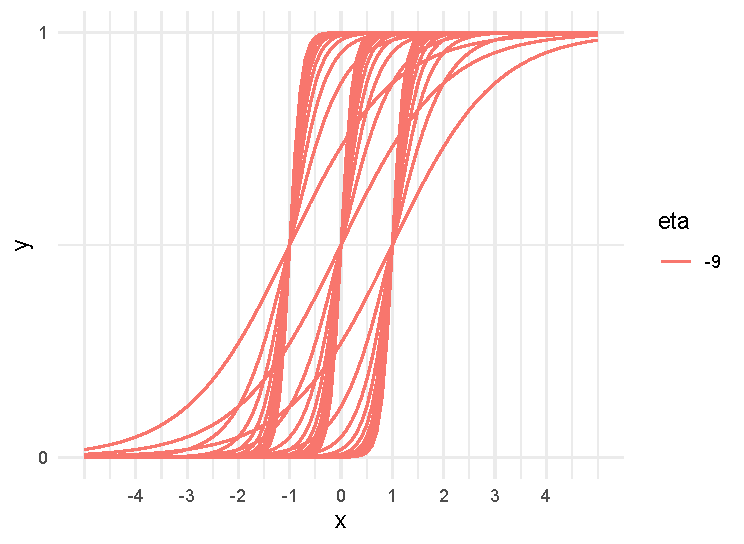
\includegraphics[width=.9\linewidth]{./images/sigmoid.pdf}
\caption{\label{fig:sigmoid}
insert caption here}
\end{figure}

Similarly to the focal loss \cite{focalLoss}, sigmoidF1 loss deals with class imbalance and robustness to outliers.

\todo{statistical robustness assessment}


% Given the presence of the step indicator function \(\sum \mathds{1}_{\mathbf{p_i} \geq b}\), \(F_\beta\) is not differentiable for gradient based methods. One way of surpassing that problem is to use a surrogate.

% \subsection{soft F1 score}
% \label{sec:org3ca83ef}

 % with smooth confusion matrix entries :



% /softF1/ is
% $$\mathcal{L}_{\text {Pred}}=\sum_{i, j}\left(\mathbf{y}_{i j}-\hat{\mathbf{y}}_{i j}\right)^{2}$$

% \subsection{sigmoidF1 score}
% \label{sec:orgc5d29d7}


% \begin{figure}[htbp]
% \centering
% 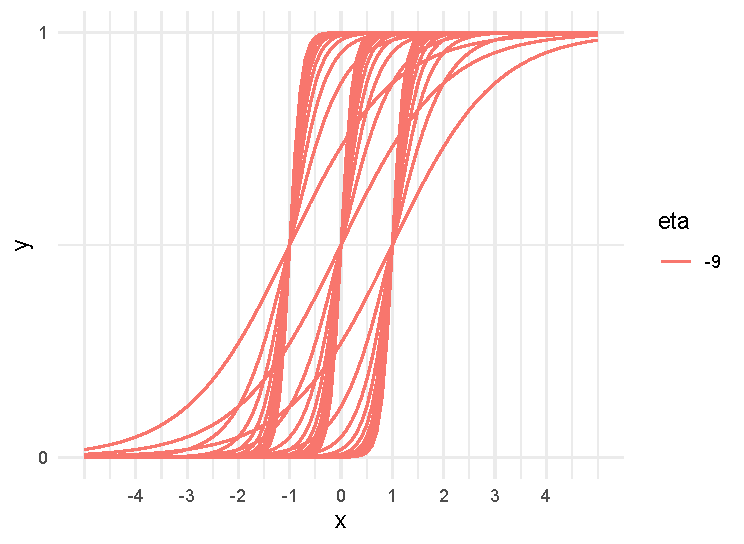
\includegraphics[width=.9\linewidth]{./images/sigmoid.pdf}
% \caption{\label{fig:sigmoid}
% Sigmoid function with different values for $\beta$ (steepness) \& $\eta$ (offset)}
% \end{figure}

%  with \(S(u)\), the confusion matrix entries then become

% \begin{equation}\label{eq:sigmoidF1}
% \widetilde{\mathit{tp}}=\sum S(\hat{\mathbf{y}}) \odot \mathbf{y} \quad\widetilde{\mathit{fp}}= \sum S(\hat{\mathbf{y}}) \odot (\mathbf{1} - \mathbf{y}) \quad \widetilde{\mathit{fn}}= \sum (\mathbf{1} - S(\hat{\mathbf{y}})) \odot \mathbf{y}
% \end{equation}

% And thus

% \begin{equation}
% \mathcal{L}_{\text {sigmoidF1}}= \frac{\widetilde{\mathit{tp}}}{2 \widetilde{\mathit{tp}}+ \widetilde{\mathit{fn}}+ \widetilde{\mathit{fp}}}
% \end{equation}

% \doubt{mention smooth hinge loss} \cite{smoothHinge}

% $\doublewidetilde{tp}$
% https://tex.stackexchange.com/questions/321231/double-widetilde
% doesn't work



\subsection{Evaluation Metrics}
\label{sec:org23c8447}

\mdr{Should this be here or in the Exp Setup section?}

The metrics described below are a result of a survey of different common practices for measuring accuracy of multilabel prediction. When true positives and false positives are used, recall that \(t p=\sum_{i \in Y^{+}} \mathds{1}_{\mathbf{p_i} \geq b}\) and \(f p=\sum_{i \in Y^{-}} \mathds{1}_{\mathbf{p_i} \geq b}\), and thus a threshold \(b\) must be set. When \(b = 0.5\), as is commonly done \todo{add source}, a risk remains that a lot of examples remain without predictions.

Extending \(F_1\) to multi-class binary classification amounts to deciding wether to un/pool classes.
In a first pooled iteration, micro \(F_1\)~\cite{multilabelMetrics} equates to creating a single 2x2 confusion matrix for all classes:
$$F_1^{micro} = \frac{\sum tp_c}{2 \sum tp_c + \sum fn_c + \sum fp_c} \quad for \quad c \in C$$

Macro \(F_1\) \cite{threshForF1, multilabelMetrics} amounts to creating one confusion matrix per class or unpooling:

$$F_1^{macro} = \frac{1}{c} \sum_{j=1}^c F_1$$

% $$F_1^{macro} = \frac{\sum tp_c}{2 \sum tp_c + \sum fn_c + \sum fp_c} \quad for \quad c \in C$$

Weighted macro \(F_1\)~\cite{weightedMetrics} is similar but includes weighing to account for class imbalance, i.e. weighing each class by the number of groundtruth positives.
\begin{equation}
F_1^{weighted} = \frac{1}{c} \sum_{j=1}^c n_j F_1 \text{ where } n_j = \sum_i \mathds{1}_{\mathbf{y_i^j} = 1}.
\end{equation}

% $$F_1^{weighted} = \frac{\sum tp_c}{2 \sum tp_c + \sum fn_c + \sum fp_c} \quad for \quad c \in C$$

We also define precision and recall

\begin{equation}
\begin{aligned} P &=\frac{t p}{t p+f p} \\ R &=\frac{t p}{t p+f n}=\frac{t p}{\left|Y^{+}\right|} \end{aligned}
\end{equation}

More variations scores exist in the literature, such as hamming loss~\cite{hammingLoss} (the fraction of incorrectly predicted labels), hamming score.

% - 'samples':
% Calculate metrics for each instance, and find their average (only meaningful for multilabel classification where this differs from accuracy_score).

% $$F_1^{micro} = \frac{\sum tp_c}{2 \sum tp_c + \sum fn_c + \sum fp_c} \quad for \quad c \in C$$

% \todo{explain batch size mathematically for F1 surrogate losses}


%%% Local Variables:
%%% mode: latex
%%% TeX-master: "../main"
%%% End:
